
% This LaTeX was auto-generated from MATLAB code.
% To make changes, update the MATLAB code and republish this document.

\documentclass{article}
\usepackage{graphicx}
\usepackage{color}

\sloppy
\definecolor{lightgray}{gray}{0.5}
\setlength{\parindent}{0pt}

\begin{document}

    
    
\subsection*{Contents}

\begin{itemize}
\setlength{\itemsep}{-1ex}
   \item part two
\end{itemize}
\begin{verbatim}
clear
close all
clc
%Lab 6
%Brian Hosler and Sarah Peachey
ce1=imread('Assignment6Files/imageCE1.tif');
ce2=imread('Assignment6Files/imageCE2.tif');
ce3=imread('Assignment6Files/imageCE3.tif');
ce4=imread('Assignment6Files/imageCE4.tif');
ce5=imread('Assignment6Files/imageCE5.tif');

subplot(1,2,1)
imhist(ce1)%ENHANCED
subplot(1,2,2)
imhist(ce2)
figure
subplot(1,2,1)
imhist(ce3)%ENHANCED
subplot(1,2,2)
imhist(ce4)

ui1=imread('Assignment6Files/unaltIm1.tif');
ui2=imread('Assignment6Files/unaltIm2.tif');
ui3=imread('Assignment6Files/unaltIm3.tif');

figure
subplot(3,1,1)
imhist(Gcorrection(ui1,.7))
subplot(3,1,2)
imhist(ui1)
subplot(3,1,3)
imhist(Gcorrection(ui1,1.3))

figure
subplot(3,1,1)
imhist(Gcorrection(ui2,.7))
subplot(3,1,2)
imhist(ui2)
subplot(3,1,3)
imhist(Gcorrection(ui2,1.3))

figure
subplot(3,1,1)
imhist(Gcorrection(ui3,.7))
subplot(3,1,2)
imhist(ui3)
subplot(3,1,3)
imhist(Gcorrection(ui3,1.3))

figure
imhist(ce5)

type('Gcorrection.m')
\end{verbatim}

        \color{lightgray} \begin{verbatim}
function [ img_out ] = Gcorrection(img_in, gama)
%Does gamma correction using the equation:
%   new=2558(old/255)^gamma
    img_out=uint8(255*(double(img_in)/255).^gama);
end

\end{verbatim} \color{black}
    
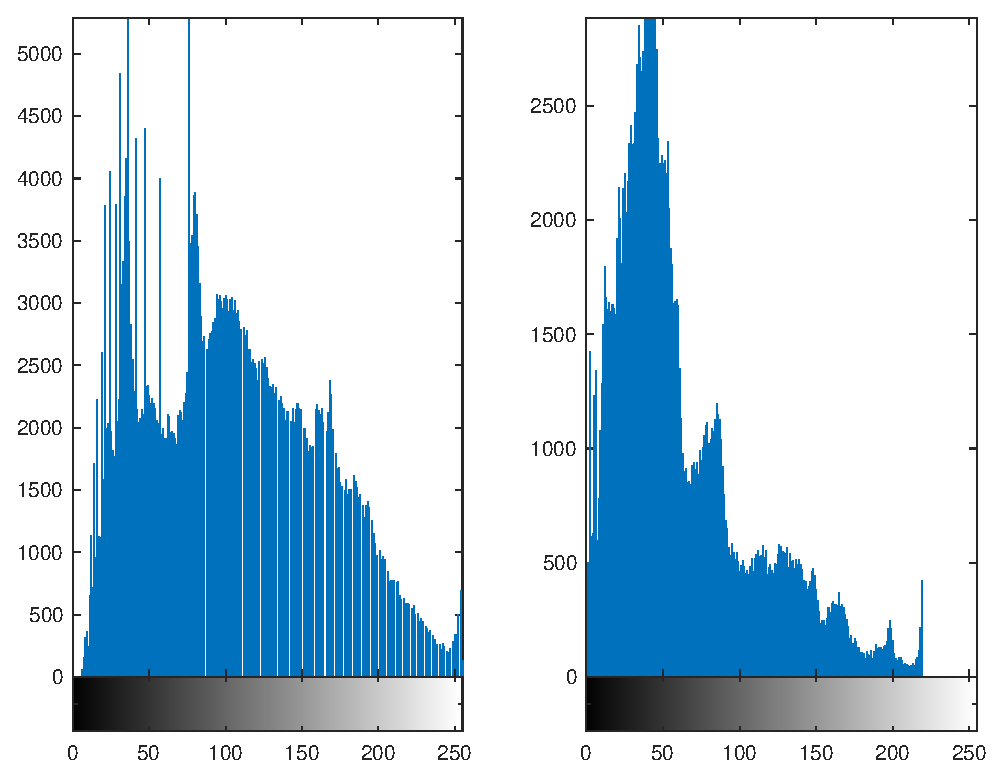
\includegraphics [width=4in]{lab6_01.eps}

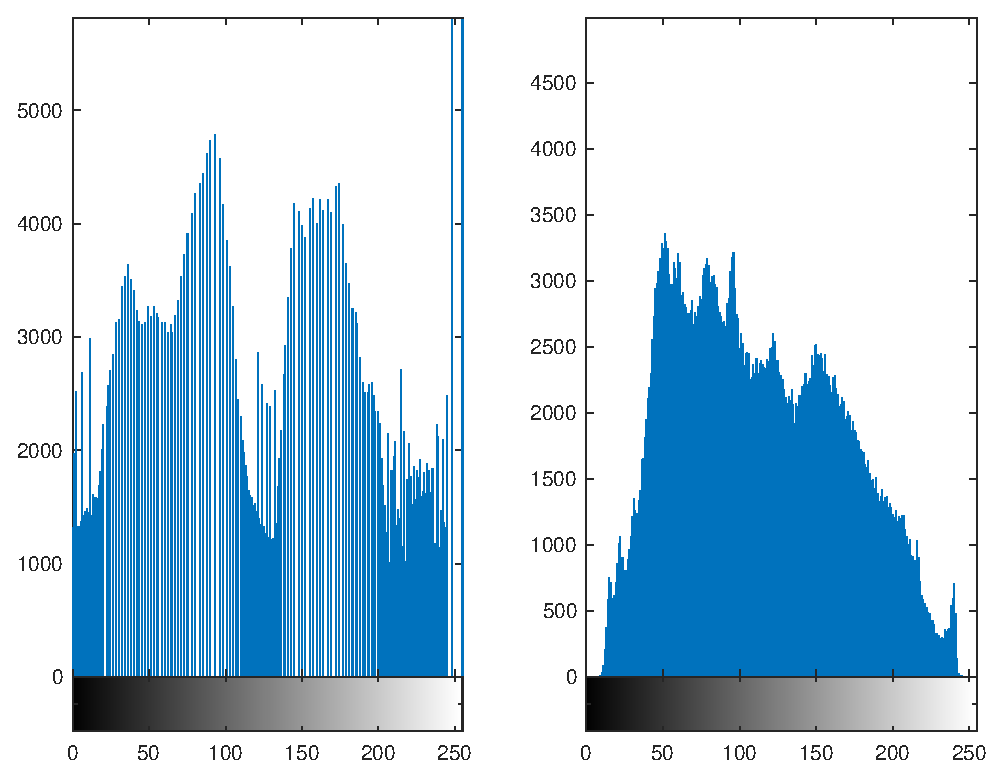
\includegraphics [width=4in]{lab6_02.eps}

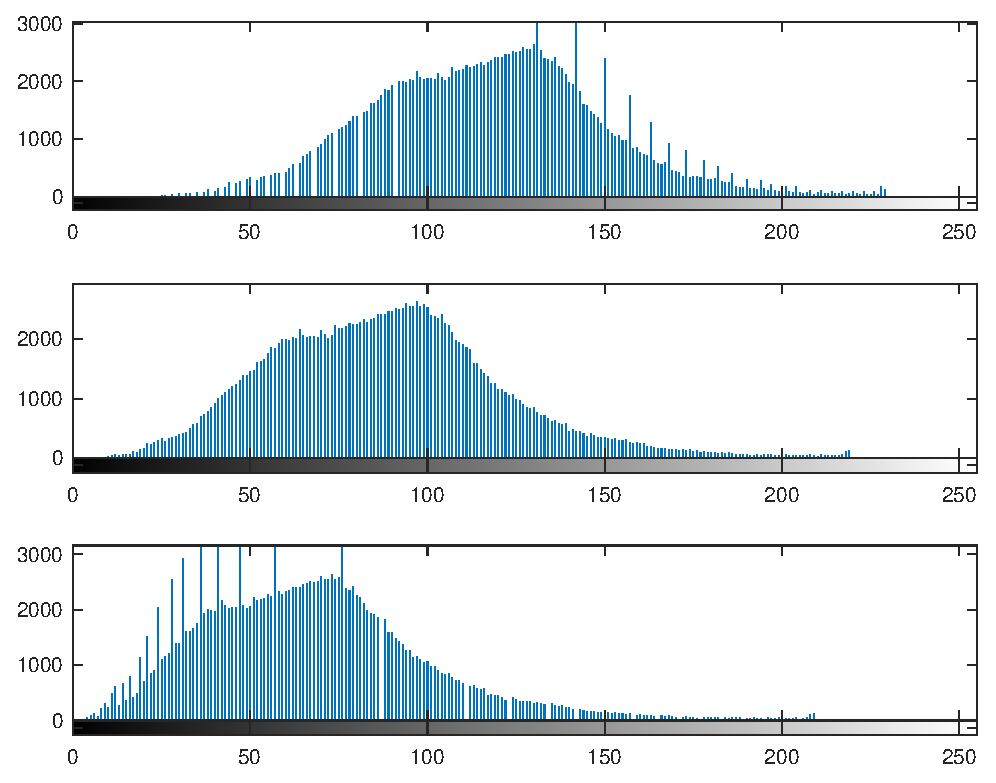
\includegraphics [width=4in]{lab6_03.eps}

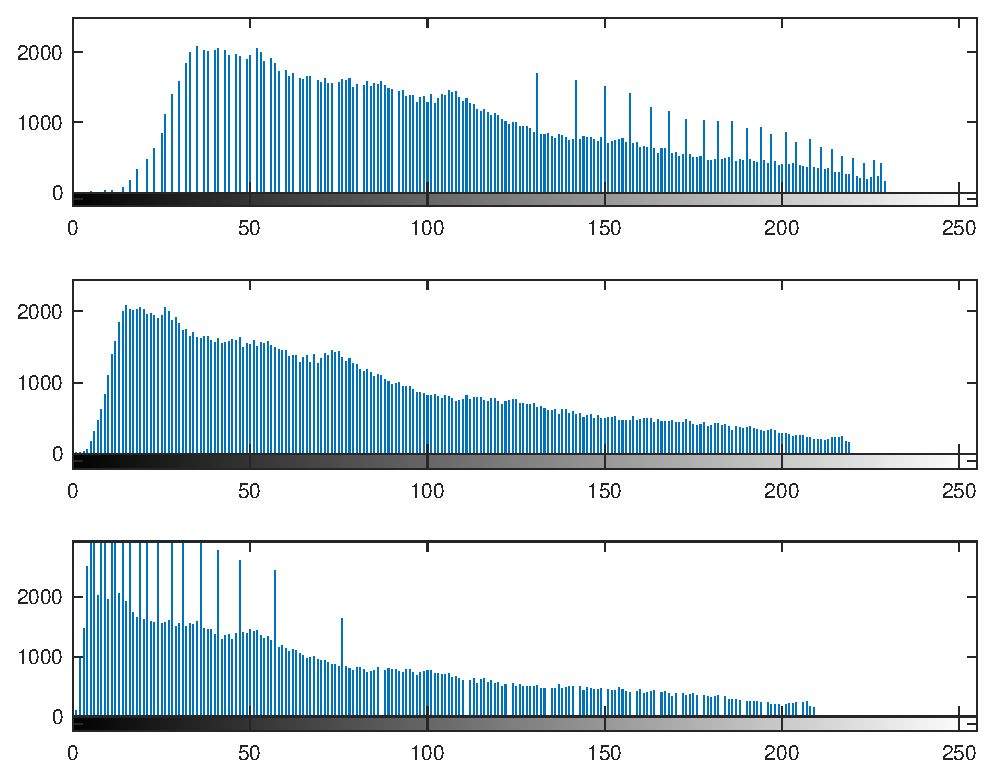
\includegraphics [width=4in]{lab6_04.eps}

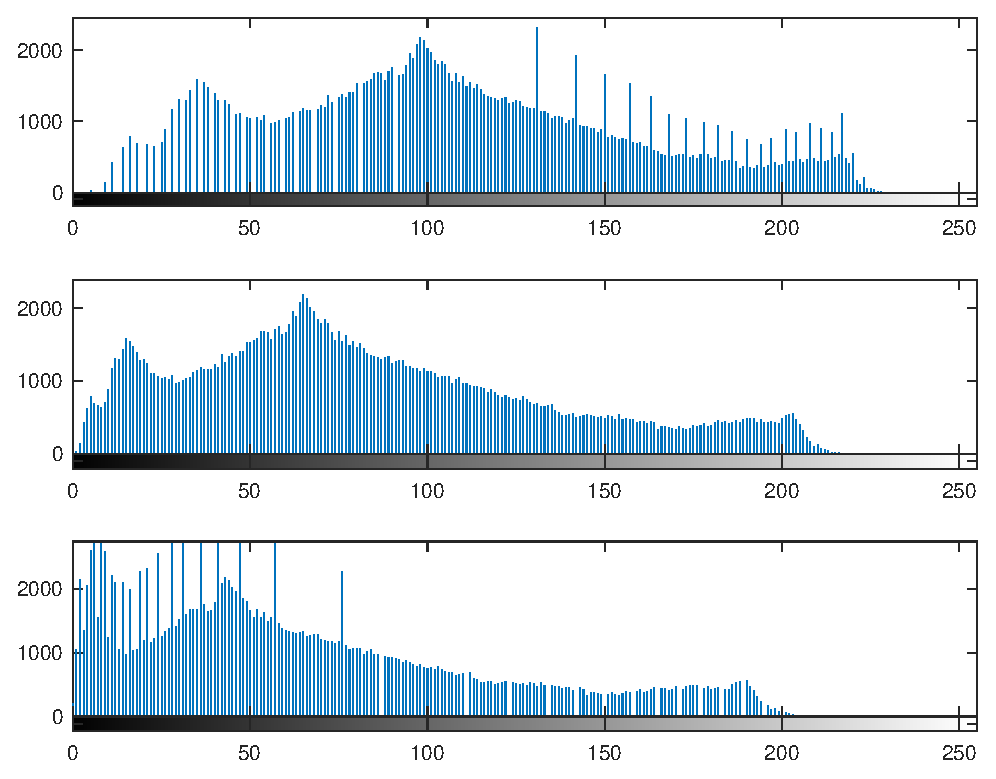
\includegraphics [width=4in]{lab6_05.eps}

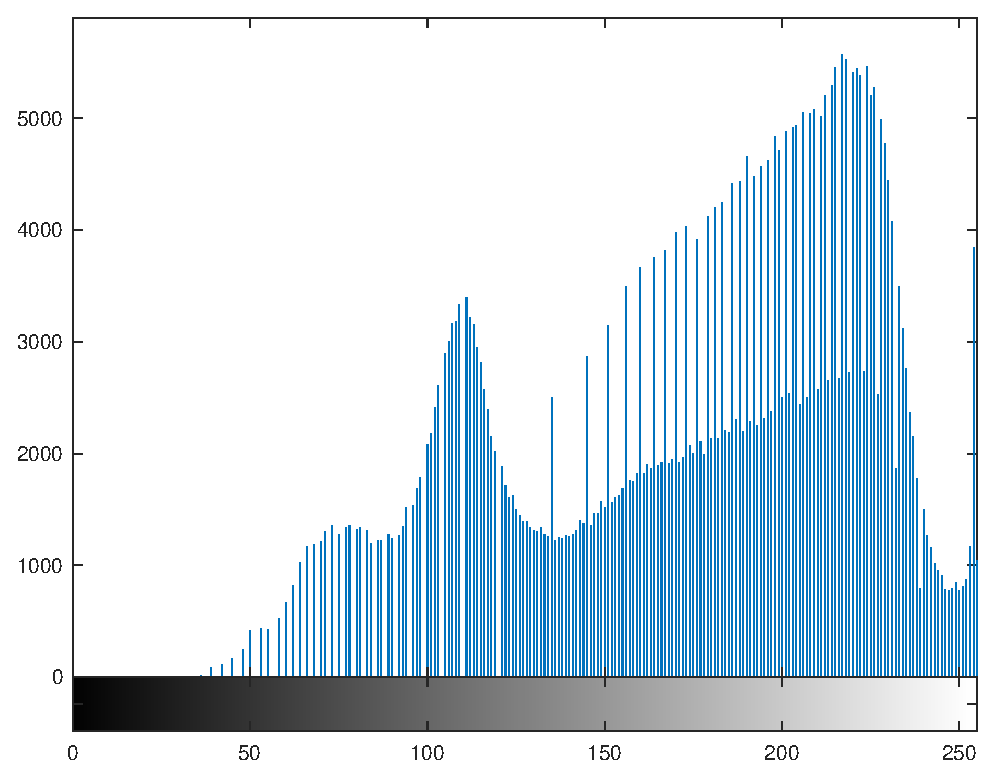
\includegraphics [width=4in]{lab6_06.eps}


\subsection*{part two}

\begin{verbatim}
im1=imread('Assignment6Files/resamp1.tif');
im2=imread('Assignment6Files/resamp2.tif');
im3=imread('Assignment6Files/resamp3.tif');
im4=imread('Assignment6Files/resamp4.tif');
p1= kirchners( im1 );
p2= kirchners( im2 );
p3= kirchners( im3 );
p4= kirchners( im4 );

figure
subplot(2,2,1)
imagesc(p1)
colormap(cool)
subplot(2,2,2)
imagesc(p2)
subplot(2,2,3)
imagesc(p3)
subplot(2,2,4)
imagesc(p4)

figure
subplot(2,2,1)
showFreqPmap(p1)
subplot(2,2,2)
showFreqPmap(p2)
subplot(2,2,3)
showFreqPmap(p3)
subplot(2,2,4)
showFreqPmap(p4)
type('kirchners.m')
\end{verbatim}

        \color{lightgray} \begin{verbatim}
function [ pmap_approx ] = kirchners( im )
%UNTITLED approximates the pmap 
%   Detailed explanation goes here
I=double(im); 
% 1)
alpha=[-0.25 0.5 -0.25; 0.5 0 0.5;-0.25 0.5 -.25]; 
I_hat=filter2(alpha, I); 
% 2)
pred_error=I-I_hat; 
% 3)
lambda=1; 
tau=2; 
sigma=1; 
pmap_approx=lambda*exp((-pred_error.^tau)./sigma); 

end

\end{verbatim} \color{black}
    
\includegraphics [width=4in]{lab6_07.eps}

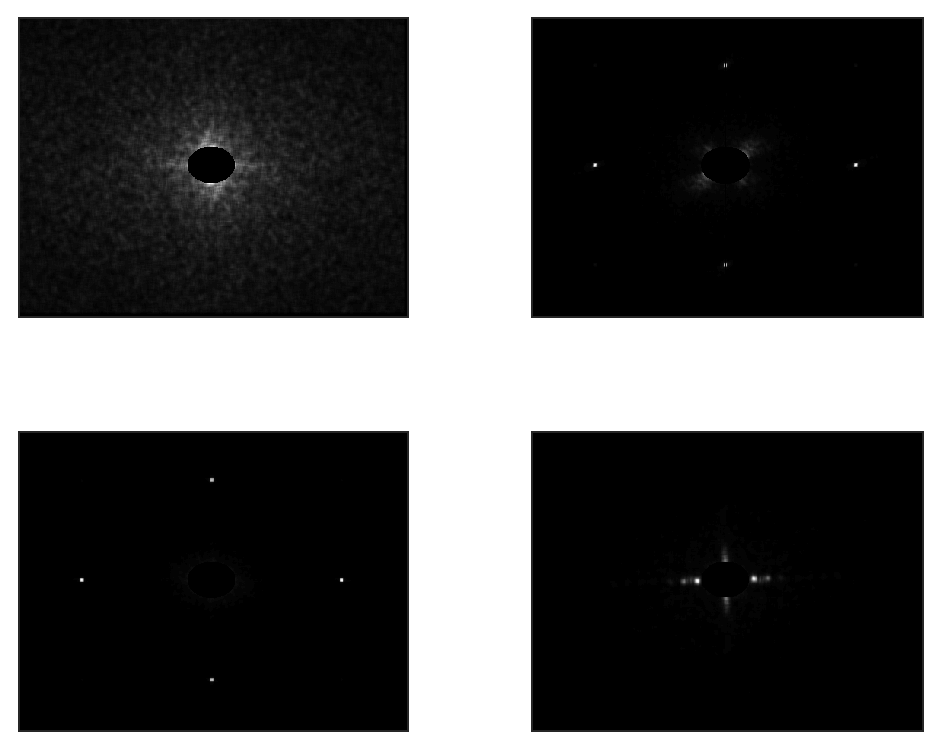
\includegraphics [width=4in]{lab6_08.eps}



\end{document}
    
